\documentclass[hyperref={pdftex,unicode}]{beamer}

\usepackage[T2A]{fontenc}
\usepackage[utf8]{inputenc}
\usepackage[russian]{babel}
\usepackage{cmap}

\usepackage{xcolor}

% \usepackage{helvet}
\usepackage{pscyr}

\usepackage{multicol}

% \usepackage{amssymb,amsfonts,amsmath,mathtext}
% \usepackage{cite,enumerate,float}

\usepackage{listings}

\graphicspath{{images/}}
\usetheme{boxes}
\usecolortheme{whale}
\useinnertheme{default}
\useoutertheme{default}
\usefonttheme{professionalfonts}

\definecolor{Blue}{RGB}{55,110,160}
\definecolor{Yellow}{RGB}{255,210,65}
\definecolor{Green}{RGB}{75,120,60}
\definecolor{LightGray}{RGB}{205,205,205}

\setbeamercolor*{palette primary}{fg=white,bg=Blue}

\setbeamercolor*{enumerate item}{fg=Yellow}
\setbeamercolor*{enumerate subitem}{fg=Yellow}
\setbeamercolor*{enumerate subsubitem}{fg=Yellow}

\setbeamercolor*{itemize item}{fg=Yellow}
\setbeamercolor*{itemize subitem}{fg=Yellow}
\setbeamercolor*{itemize subsubitem}{fg=Yellow}

\lstset{
  language=python,
  basicstyle=\small\ttfamily,
  keywordstyle=\bfseries\color{Blue},
  commentstyle=\color{Green},
  numberstyle=\footnotesize\color{LightGray},
  numbersep=0.8em,
  stepnumber=1,
  keepspaces=true,
  breaklines=true,
  aboveskip=0.5\baselineskip,
  belowskip=0.5\baselineskip}


\title{Python: functions}
\author{meequz@gmail.com \\ budnyjj@pirates.by}
\date{}

\begin{document}

\begin{frame}
  \maketitle
\end{frame}

\begin{frame}{Об авторе этих слайдов}
  \begin{minipage}{0.3\linewidth}
    \begin{figure}[H]
      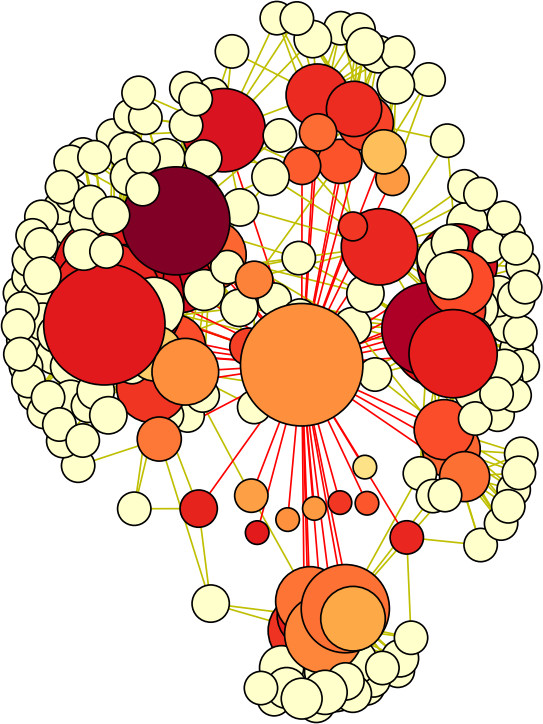
\includegraphics[width=1\linewidth]{my_logo.jpg}
    \end{figure}
  \end{minipage}
  \hfill
  \begin{minipage}{0.6\linewidth}
    Меня зовут Роман. 
    
    Я студент четвертого курса БГУИР.

    Постоянно использую python для:
    \begin{itemize}
      \item учебы
      \item работы
      \item развлечения
    \end{itemize}
  \end{minipage}
\end{frame}

\begin{frame}{Этот курс может быть полезен для \dots}
  \begin{itemize}
    \item желающих научиться программировать
    \item студентов технических специальностей
    \item системных администраторов
    \item ...
  \end{itemize}
\end{frame}

\begin{frame}{Программа курса}
  \begin{minipage}{0.4\linewidth}
    \begin{itemize}
    \item Базовые типы
    \item Контейнеры
    \item Функции
    \item Классы
    \item Исключения
    \end{itemize}
  \end{minipage}
  $ \Longrightarrow $
  \hfill
  \begin{minipage}{0.4\linewidth}
    \begin{itemize}  
    \item 8 лекционных часов
    \item задачи на дом
   \end{itemize}
  \end{minipage}
\end{frame}

\begin{frame}{Сегодня}
  \begin{itemize}
  \item Обзор языка
  \item Hello, world!
  \item Базовые типы данных
  \item Условный оператор
  \item Операторы цикла
  \end{itemize}
\end{frame}

\begin{frame}{Python}
  Python --- язык программирования общего назначения,
  ориентированный на повышение производительности разработчика и читаемости кода.
\end{frame}

\begin{frame}{Название языка}
  Автор назвал язык в честь британского комедийного телешоу 1970-х
  <<Летающий цирк Монти Пайтона>>.

  \begin{figure}[H]
    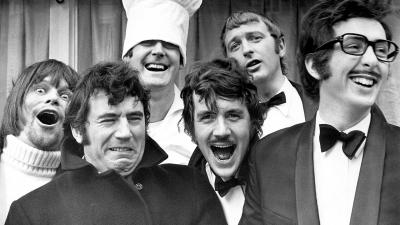
\includegraphics[width=0.8\linewidth]{python.jpg}
  \end{figure}
\end{frame}

\begin{frame}{Особенности языка Python}
  \begin{itemize}
    \item Интерпретируемый
    \item Высокоуровневый
    \item Динамически типизируемый
    \item Поддерживает ООП
  \end{itemize}
\end{frame}

\begin{frame}{Версии Python}
  \centering
  ``Python 2.x is legacy, \\
  Python 3.x is the present
  and future of the language'' \footnote[frame]{
    https://wiki.python.org/moin/Python2orPython3}
\end{frame}

\begin{frame}{Getting help}
  \begin{itemize}
    \item https://docs.python.org
    \item opennet.ru/docs/RUS/python/
    \item help()
  \end{itemize}
\end{frame}

\begin{frame}[fragile]{Hello, world!}
  \begin{itemize}
  \item Interactive
    \begin{lstlisting}
python
>>> print "Hello, world!"
    \end{lstlisting}
  \item Script hello.py:
    \begin{lstlisting}[numbers=left]
#!/usr/bin/python2
print "Hello, world!"
    \end{lstlisting}

  \begin{minipage}{0.4\linewidth}
     \begin{lstlisting}[language=bash]
chmod +x hello.py
./hello.py
     \end{lstlisting}
   \end{minipage}
   \hfill or \hfill
   \begin{minipage}{0.4\linewidth}
     \begin{lstlisting}[language=bash]
python2 hello.py
     \end{lstlisting}
   \end{minipage}

  \end{itemize}
\end{frame}

\begin{frame}[fragile]{import this}
  \begin{center}
    \texttt{python -c "import this"}
  \end{center}
\end{frame}

\begin{frame}{Zen of Python}
\footnotesize{
Красивое лучше, чем уродливое.

Явное лучше, чем неявное.

Простое лучше, чем сложное.

Сложное лучше, чем запутанное.

Плоское лучше, чем вложенное.

Разреженное лучше, чем плотное.

Читаемость имеет значение.

Особые случаи не настолько особые, чтобы нарушать правила.

При этом практичность важнее безупречности.

Ошибки никогда не должны замалчиваться.

Если не замалчиваются явно.

Встретив двусмысленность, отбрось искушение угадать.

Должен существовать один --- и, желательно, только один — очевидный способ сделать это.

Хотя он поначалу может быть и не очевиден, если вы не голландец.

Сейчас лучше, чем никогда.

Хотя никогда зачастую лучше, чем прямо сейчас.

Если реализацию сложно объяснить — идея плоха.

Если реализацию легко объяснить — идея, возможно, хороша.

Пространства имён — отличная штука! Будем делать их побольше!}
\end{frame}

\begin{frame}{Идентификаторы}
  \begin{itemize}
    \item A-Z, a-z, 0-9, \_
    \item Case sensitive
  \end{itemize}
\end{frame}

\begin{frame}{Стандартные типы данных}
  \begin{itemize}
    \item Boolean
    \item Numeric: int, float, long, complex
    \item String
    \item List
    \item Tuple
    \item Dictionary\footnote[frame]{
        Существуют различия в типах данных в разных версиях Python: \\
        https://docs.python.org/2.7/library/stdtypes.html \\
        https://docs.python.org/3.4/library/stdtypes.html}
  \end{itemize}
\end{frame}

\begin{frame}[fragile]{Базовые типы данных}
  \begin{lstlisting}[numbers=left]
#!/usr/bin/python

logic   = True         # A boolean assignment
counter = 103          # An integer 
miles   = 1000.0       # A floating point
cmplx   = 1 + 1j       # A complex 
name    = "John"       # A string

print logic, not Logic
print counter, counter * miles
print miles, miles / counter, miles // counter
print cmplx, cmplx.conjugate()
print name, "|".join(name)
\end{lstlisting}
\end{frame}

\begin{frame}[fragile]{Преобразование типов}
  \begin{lstlisting}[numbers=left]
type(x)
int(x[, base])
long(x[, base])
float(x)
complex(real[,imag])
str(x)
repr(x)
eval(x)
chr(x)
unichr(x)
ord(x)
\end{lstlisting}
\end{frame}

\begin{frame}[fragile]{Операторы}
\begin{lstlisting}
+, -, *, /, %, **, //    # arithmetical
==, !=, <, >, >=, <=     # comparison
and, or, not             # logical
in                       # membership
is                       # identity
\end{lstlisting}
\end{frame}

\begin{frame}[fragile]{Пара слов про контейнеры}
  \begin{itemize}
    \item List
      \begin{lstlisting}[numbers=left]
l = [1, 2]
l.append(3)
print l
l.append(l)
print l
      \end{lstlisting}
    \item Dict
      \begin{lstlisting}[numbers=left]
d = {"one": 1, "two": 2,}
d["three"] = 3
print d
del(d["two"]
print d
      \end{lstlisting}
  \end{itemize}
\end{frame}

\begin{frame}[fragile]{Примечания}
  \begin{itemize}
    \item Boolean, Numeric, Complex, String, Tuple are \textbf{immutable}
    \item List, Dictionary are \textbf{mutable}
    \item \lstinline$'foo' == "foo"$
    \item Docstring:
      \begin{lstlisting}
"""
This is a docstring example.

It is useful mainly for documentation purposes.
"""
      \end{lstlisting}
  \end{itemize}
\end{frame}

\begin{frame}[fragile]{Условный оператор}
  \begin{lstlisting}[numbers=left]
x = int(raw_input("Please enter an integer: "))
if x < 0:
    x = 0
    print "Negative changed to zero"
elif x == 0:
    print "Zero"
elif x == 1:
    print "Single"
else:
    print "More"
  \end{lstlisting}
\end{frame}

\begin{frame}[fragile]{Оператор цикла for}
  \begin{lstlisting}[numbers=left]
words = ["cat", "window", "defenestrate"]
for w in words:
    print w, len(w)

# range(5)         == [0, 1, 2, 3, 4]
# range(3,10)      == [3, 4, 5, 6, 7, 8, 9]
# range(3, 10, 2)  == [3, 5, 7, 9]
# range(3, 10, -2) == [9, 7, 5, 3]

for i in range(len(words)):       # ugly
    print i, words[i]

for i, word in enumerate(words):  # much better
    print i, word

\end{lstlisting}
\end{frame}

\begin{frame}[fragile]{Оператор цикла for}
  \begin{lstlisting}[numbers=left]
for n in range(2, 10):
     for x in range(2, n):
         if n % x == 0:
             print n, "equals", x, "*", n/x
             break
     else:
         print n, "is a prime number"
  \end{lstlisting}
\end{frame}

\begin{frame}[fragile]{Оператор цикла for}
  \begin{lstlisting}[numbers=left]
for num in range(2, 10):
    if num % 2 == 0:
         print "Found an even number", num
         continue
    print "Found a number", num
  \end{lstlisting}
\end{frame}

\begin{frame}[fragile]{Оператор цикла while}
  \begin{lstlisting}[numbers=left]
while True:
    pass
  \end{lstlisting}
\end{frame}

\begin{frame}[fragile]{import math}
\begin{lstlisting}[numbers=left]
import math
dir(math)
help(math)
\end{lstlisting}
\end{frame}

\begin{frame}[fragile]{Пример решения задачи \\ <<найти n-тоe число Фибоначчи>>\footnote[frame]{
http://stackoverflow.com/questions/494594/how-to-write-the-fibonacci-sequence-in-python}}
\begin{equation*}
  F_n = \left\{
    \begin{array}{l l}
      0 & \quad \text{при n = 0;}\\
      1 & \quad \text{при n = 1;}\\
      F_{n-1} + F_{n-2} & \quad \text{при n > 1.}
    \end{array} \right.
\end{equation*}
\smallskip

\begin{lstlisting}[basicstyle=\footnotesize\ttfamily,numbers=left]
def fib(n):
""" Return n-th number in Fibonacci sequence. """
    if n == 0: return 0
    elif n == 1: return 1
    else: return fib(n-1) + fib(n-2)

reqNumber = int(raw_input(
"Enter index of requested Fibonacci number: "))
print("Your number is:", fib(reqNumber))
\end{lstlisting}
\end{frame}

\begin{frame}{Задача <<n-тоe число Фибоначчи>>}
  \begin{itemize}
  \item Что будет, если мы попытаемся вычислить fib(-1)?
  \item Можно ли оптимизировать процесс вычислений? \\ Как это сделать?
  \end{itemize}
\end{frame}

\begin{frame}{Спасибо за внимание!}
  Репозиторий курса находится здесь: \\
  https://github.com/budnyjj/courses\_python

\end{frame}


\end{document}